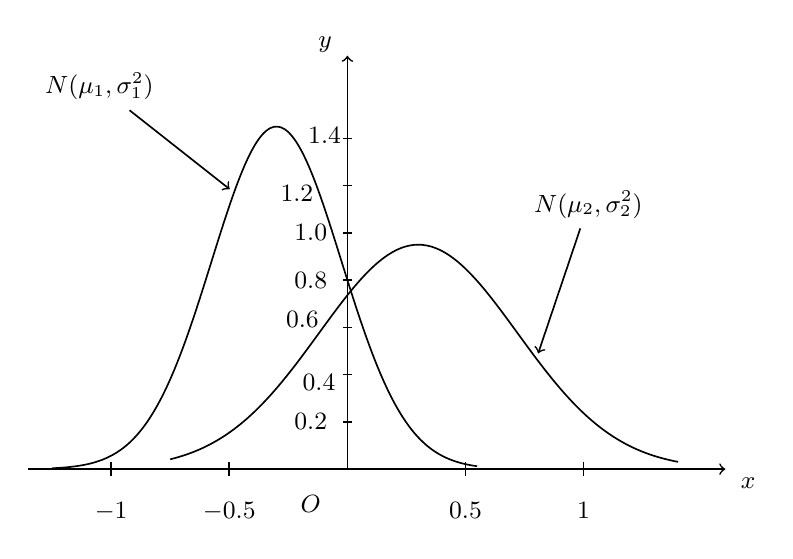
\begin{tikzpicture}[line width=0.6pt, font=\small, x=3cm, y=3cm]
% axes
\draw[->] (-1.35,0) -- (1.6,0) node[below=5pt,right=2pt] {$x$};
\draw[->] (0,0) -- (0,1.75) node[above=4pt,left=2pt] {$y$};
% x ticks
\foreach \x/\lbl in {-1/$-1$, -0.5/$-0.5$, 0.5/$0.5$, 1/$1$} {
  \draw (\x,0.03) -- (\x,-0.03);
  \node[below=6pt] at (\x,-0.03) {\lbl};
}
\node[below left=6pt] at (0,0) {$O$};
% y ticks
\draw (0.02,0.2) -- (-0.02,0.2);
\node[left=2pt] at (-0.02,0.2) {$0.2$};
\draw (0.02,0.4) -- (-0.02,0.4);
\node[left=2pt,xshift=3pt,yshift=-3pt] at (-0.02,0.4) {$0.4$};
\draw (0.02,0.6) -- (-0.02,0.6);
\node[left=2pt,xshift=-3pt,yshift=3pt] at (-0.02,0.6) {$0.6$};
\draw (0.02,0.8) -- (-0.02,0.8);
\node[left=2pt] at (-0.02,0.8) {$0.8$};
\draw (0.02,1.0) -- (-0.02,1.0);
\node[left=2pt] at (-0.02,1.0) {$1.0$};
\draw (0.02,1.2) -- (-0.02,1.2);
\node[left=2pt,xshift=-5pt,yshift=-3pt] at (-0.02,1.2) {$1.2$};
\draw (0.02,1.4) -- (-0.02,1.4);
\node[left=2pt,xshift=5pt,yshift=1pt] at (-0.02,1.4) {$1.4$};
% normal curves from Gaussian formula
\draw[solid, domain=-1.25:0.55, samples=120, smooth]
  plot (\x, {1.45*exp(-((\x+0.30)^2)/(2*0.275132607173^2))});
\draw[solid, domain=-0.75:1.40, samples=120, smooth]
  plot (\x, {0.95*exp(-((\x-0.30)^2)/(2*0.419939242528^2))});
% curve labels with clearance
\node (L1) at (-1.05,1.62) {$N(\mu_{1},\sigma_{1}^{2})$};
\draw[->,shorten >=2pt] (L1) -- (-0.48,1.170643265956);
\node (L2) at (1.02,1.12) {$N(\mu_{2},\sigma_{2}^{2})$};
\draw[->,shorten >=2pt] (L2) -- (.8,0.467623357639);
\end{tikzpicture}
